\documentclass{article}
\usepackage{tikz}
\begin{document}

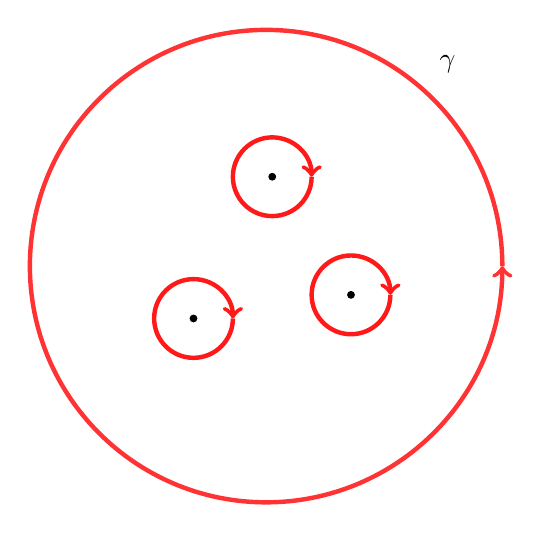
\begin{tikzpicture}
	\coordinate (A) at (0, 0);
	\coordinate (B) at (1,1.8);
	\coordinate (C) at (2, .3);
	\foreach \n in {(A), (B), (C)}
		\draw[color=red!90, ultra thick, ->] \n ++ (0:.5) arc (360:0:.5);
	\foreach \n in {(A), (B), (C)}
		\node at \n [circle,fill,inner sep=1pt]{};
	\draw[color=red!80, ultra thick, ->] (0.922, 0.665)  ++ (0: 3) arc (0:360: 3);
	\node[above right] at (3, 3) {$\LARGE{\gamma}$};
\end{tikzpicture}

\end{document}
